\section{Introduction}
\subsection{Hybrid systems}
\begin{frame}{What is an hybrid system?}
Computer sciences are used to deal with discrete objects.
image

Discrete models are not always adapted to the continuous world of physic quantities.
image

An hybrid system mixes both. Their study is crucial and difficult.
image

\end{frame}

\begin{frame}{A model: the hybrid automaton}
\begin{columns}[c]

\begin{column}{5cm}
heater example
\end{column}

\begin{column}{5cm}
It is composed by:
\begin{itemize}
\item a set of discrete states;
\item a set of continuous variables, controlled by the discrete states;
\item conditions on the variables to stay in the current state;
\item transitions between the discrete states, with reassignments and conditions over the variables.
\end{itemize}
\end{column}


\end{columns}

\vspace*{1cm}

A state = a discrete state + a valuation for the variables.
\end{frame}

\subsection{Model checking of an Hybrid automaton}
\begin{frame}{The reachability analysis}
There are several methods to ensure the safety of an hybrid automaton:
\begin{itemize}
\item theorem proving;
\item interval based methods;
\item flowpipe computation.
\end{itemize}
\begin{block}{Flowpipe computation}
The behaviour of the variables is described by a differential equation. An analytic solution can be found for a given set of times. A polyhedron over approximates the variables between two analytical points.
\end{block}
\begin{figure}
\includegraphics[scale=1]{images/flowpipe1.eps}
\hspace*{1.5cm}

\includegraphics[scale=1]{images/flowpipe2.eps}
\hspace*{1.5cm}

\includegraphics[scale=1]{images/flowpipe3.eps}
\caption{Construction of a polyhedron during flowpipe computation.}
\end{figure}

\end{frame}

\begin{frame}{Two kind of polyhedra}
Key issue for flowpipe computation: being able to manipulate these polyhedra. There are two kind of polyhedra:
\only<2,3>{\begin{block}{$V$-polyhedron}
A $V$-polyhedron $P$ is the Minkowsky sum of the convex hull of a set $V$ of vertices and the conic hull of a set $C$ of vectors. $P= conv(V) + cone(C)$.
\end{block}}
\only<3>{
\begin{figure}
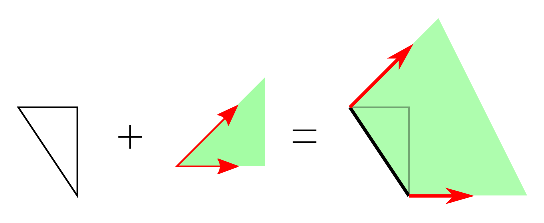
\includegraphics[scale=1]{images/vpoly.eps}
\caption{Construction of a $V$-polytope}
\end{figure}
}


\only<4,5>{\begin{itemize}
\item the $V$-polyhedron;
\end{itemize}
\begin{block}{$H$-polyhedron}
An $H$-polyhedron $P$ is the intersection of a set of half-spaces: $\cap_{i=0}^n\{ x|a_i.x\leq b_i \}$. This can be written with a matrix $\{ x| Ax \leq b\}$.
\end{block}}
\only<5>{
\begin{figure}
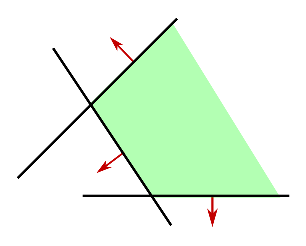
\includegraphics[scale=0.6]{images/hpoly.eps}
\caption{Construction of a $H$-polytope}
\end{figure}
}
\visible<6,7,8>{
\begin{itemize}
\item the $V$-polyhedron;
\item the $H$-polyhedron.
\end{itemize}
\begin{table}
\centering
\begin{tabular}{| c | c | c | c |}
	\hline	
				    & $.\ \cap\ .$ & $.\ \cup\ .$ & $.\ +\ .$ \\ \hline
	$V$-Polyhedra   & $-$ & $+$ & $+$ \\ \hline
   	$H$-Polyhedra   & $+$ & $-$ & $-$\\ \hline
\end{tabular}
\caption{Comparison of the two representations.}
\end{table}
\vspace*{-0.5cm}
}

\visible<7,8>{\begin{block}{Central theorem of polyhedra representation}
A subset $P$ of $\mathbb{R}^d$ is a $V$-polyhedron if and only if it is an $H$-polyhedron.
\end{block}}
\visible<8>{The internship resulted in a contribution to HyPro.}
\end{frame}

\begin{frame} 
	\begin{center}{\Large Plan }\end{center}
	\tableofcontents
\end{frame}





